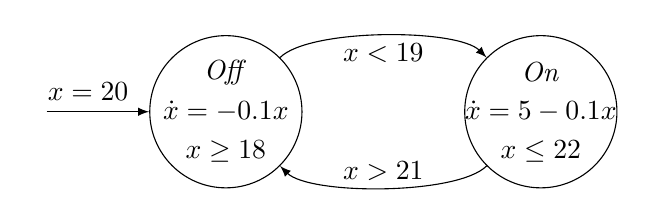
\begin{tikzpicture}[>=latex]
   
  \begin{scope}

%   \draw  (1,1) rectangle (7,1.5);

%\filldraw[black] (0,0) circle (2pt) node[anchor=west] {s};

  \node[circle, inner sep=2pt,draw, minimum height=55pt] (p1) at (-4,0) {};
      \node (p0_d) at (-4.0,0.5) {\textit{Off}};
      \node (p0_d) at (-4.0,0) {$\dot{x}=-0.1x$};
      \node (p0_d) at (-4.0,-0.5) {$x \geq 18$};
  
  \node[circle, inner sep=2pt,draw, minimum height=55pt] (p2) at (0,0) {};
      \node (p0_d) at (0.0,0.5) {\textit{On}};
      \node (p0_d) at (0.0,0) {$\dot{x}=5-0.1x$};
      \node (p0_d) at (0.0,-0.5) {$x \leq 22$};
  
     \draw[->] (p1) .. controls +(45:1.5) and +(135:1.5) .. (p2);
     \node (p0_d) at (-2.0,-0.75) {$x > 21$};
     
      \draw[->] (p2) .. controls +(-135:1.5) and +(-45:1.5) .. (p1);
      \node (p0_d) at (-2.0,0.75) {$x < 19$};
      
      
      \node (p0t) at (-5.75,0.25) {$x=20$};
      \node (p0) at (-6.40,-0.0) {};
        \draw[->] (p0) edge (p1);  
      
%       \draw[->] (p2) edge [loop right] node {} (p2);  
     
%     \node[circle, inner sep=2pt,draw, minimum height=20pt](p3) at (0.25,3) {on}; 
%     \node[circle, inner sep=2pt,draw, minimum height=20pt](p4) at (-0.5,1.5) {$\text{int}_2$}; 
%     
%     \node (p0_d) at (1.2,0) {$\inv:\dot T=0$};

  
%   \node (p0_d) at (1,1.8) {pre$_{\vdash}\cup$ pre$_{\vdash}^{\num}$};
%   \node (p1_d) at (4,1.8) {pre$_{\leftrightarrow}\cup$ pre$_{\leftrightarrow}^{\num}$};
%   \node (p2_d) at (7,1.8) {pre$_{\dashv}\cup$ pre$_{\dashv}^{\num}$};
% 
%   \node (p3_d) at (1.2,0.7) {eff$_{\vdash}^+\cup$ eff$_{\vdash}^-\cup$ eff$_{\vdash}^{\num}$};
%   \node (p5_d) at (4,0.7) {eff$_{\leftrightarrow}^{\num}$};
%   \node (p6_d) at (6.8,0.7) {eff$_{\dashv}^+\cup$ eff$_{\dashv}^-\cup$ eff$_{\dashv}^{\num}$};
% 
%     \node (p7_d) at (4,1.25) {$A$};
%   
  \end{scope}
\end{tikzpicture}